% Test tex file!

\documentclass[UTF8]{ctexart}
% \documentclass[a4paper,12pt]{article}
\usepackage{times}  % DO NOT CHANGE THIS
\usepackage{helvet} % DO NOT CHANGE THIS
\usepackage{courier}  % DO NOT CHANGE THIS
\usepackage[hyphens]{url}  % DO NOT CHANGE THIS
\usepackage{graphicx} % DO NOT CHANGE THIS
\urlstyle{rm} % DO NOT CHANGE THIS
\def\UrlFont{\rm}  % DO NOT CHANGE THIS
\usepackage{natbib}  % DO NOT CHANGE THIS AND DO NOT ADD ANY OPTIONS TO IT
\usepackage{caption} % DO NOT CHANGE THIS AND DO NOT ADD ANY OPTIONS TO IT
\frenchspacing  % DO NOT CHANGE THIS
\setlength{\pdfpagewidth}{8.5in}  % DO NOT CHANGE THIS
\setlength{\pdfpageheight}{11in}  % DO NOT CHANGE THIS
\usepackage{algorithm} %format of the algorithm 
\usepackage{algorithmic} %format of the algorithm 
\usepackage{multirow} %multirow for format of table 
\usepackage{amsmath} 
\usepackage{xcolor}
\usepackage{amssymb}
\usepackage{amsmath}
\usepackage{CJKutf8}
\usepackage{courier}

\begin{document}
% \begin{CJK}{UTF8}{gbsn}
% \begin{CJK}{UTF8}{gkai}

\title{强化学习:作业一}

\author{张含笑 502022370062}

\date{\today}

\maketitle

\section{作业内容}
在“蒙特祖马的复仇”环境中实现Dagger算法。


\section{实现过程}

首先...然后...


\section{复现方式}
在主文件夹下运行 \texttt{python main.py}.


\section{实验效果}

% 见图 \ref{performance}。描述累计奖励、访问专家次数和样本训练量之间的关系。

% \begin{figure}[h!]
% \centering
% 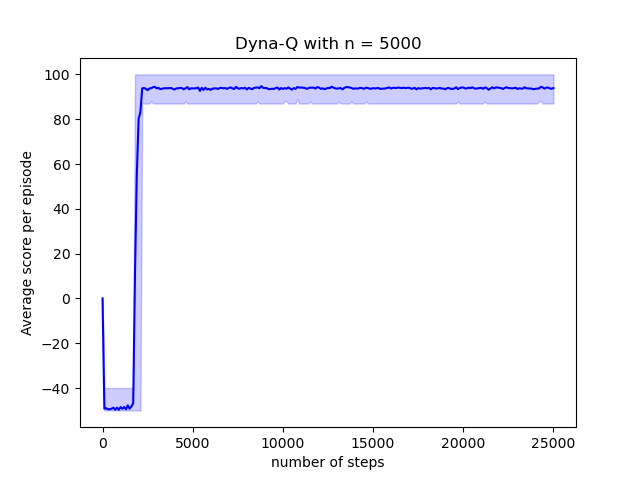
\includegraphics[width=8cm,height=7cm]{performance.png}
% \caption{Dagger算法}
% \label{performance}
% \end{figure}


\section{小结}
在这次实验中,我发现...



% \end{CJK}
\end{document}